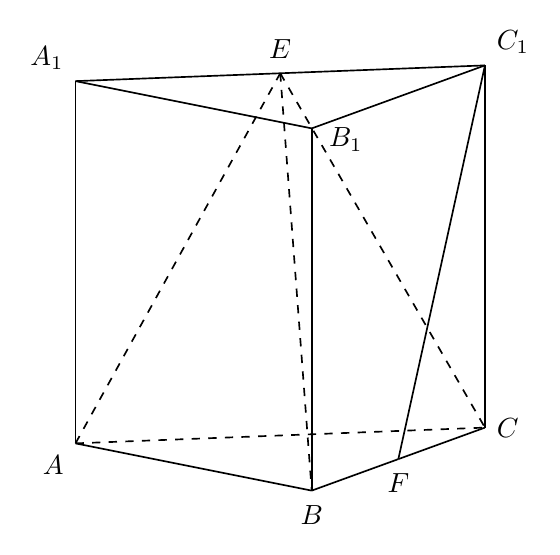
\begin{tikzpicture}[line width=.6pt]
\coordinate (A) at (0,0);
\coordinate (B) at (3,-0.6);
\coordinate (C) at (5.2,0.2);
\coordinate (A1) at (0,4.6);
\coordinate (E) at (2.6,4.7);
\coordinate (C1) at (5.2,4.8);
\coordinate (B1) at (3,4);
\coordinate (F) at (4.1,-0.2);
% solid visible edges
\draw (A1) -- (A);
\draw (A1) -- (E);
\draw (E) -- (C1);
\draw (A1) -- (B1);
\draw (C1)--(B1);
\draw (C1)--(C);
\draw (B1) -- (B);
\draw (A) -- (B);
\draw (B) -- (F);
\draw (F) -- (C);
\draw (C1) -- (F);
% hidden / auxiliary dashed edges
\draw[dashed] (A) -- (C);
\draw[dashed] (A) -- (E);
\draw[dashed] (E) -- (B);
\draw[dashed] (E)--(C);
% labels offset to avoid touching strokes
\node[fill=none,inner sep=1pt,above left=3pt] at (A1) {$A_{1}$};
\node[fill=none,inner sep=1pt,above=4pt] at (E) {$E$};
\node[fill=none,inner sep=1pt,above right=3pt] at (C1) {$C_{1}$};
\node[fill=none,inner sep=1pt,right=3pt,xshift=2.00bp,yshift=-4.00bp] at (B1) {$B_{1}$};
\node[fill=none,inner sep=1pt,below left=3pt] at (A) {$A$};
\node[fill=none,inner sep=1pt,below=4pt] at (B) {$B$};
\node[fill=none,inner sep=1pt,right=3pt] at (C) {$C$};
\node[fill=none,inner sep=1pt,below=4pt] at (F) {$F$};
\end{tikzpicture}
